\include{tex/headerueb}
\include{tex/header}
\include{tex/info}

\newcommand{\nr}{2}
\lstset{language=matlab}

\begin{document}
\section*{Aufgabe 1 - Rotationserkennung}
Wie bereits ausf\"uhrlich im Tutorium und in der Vorlesung beschrieben, f\"uhrten wir f\"ur die
L\"osung folgende Schritte durch:

\begin{enumerate}
\item Einlesen\ldots
\item Durchf\"uhrung der FFT: $T = fft( fft(I)^{T} )^{T}$
\item Beachte: Transponierung um Orientierung beizubehalten
\item Shiften des transfomrierten Bildes, um tiefen Frequenzen zu zentrieren
\item die tiefsten Frequenzen (Mittelwerte) auf Null setzen 
      (kleine Fl\"ache in der Mitte des Bildes)
\item per $[colmax, irow] = max(T)$ und $[max, icol] = max(colmax)$ den gr\"ossten Werd der
      verbleibenden Elemente finden
\item triviale Trigonometrie f\"ur Winkel und Abstand anwenden
\end{enumerate}

%\begin{figure}[H]
%\begin{center}
%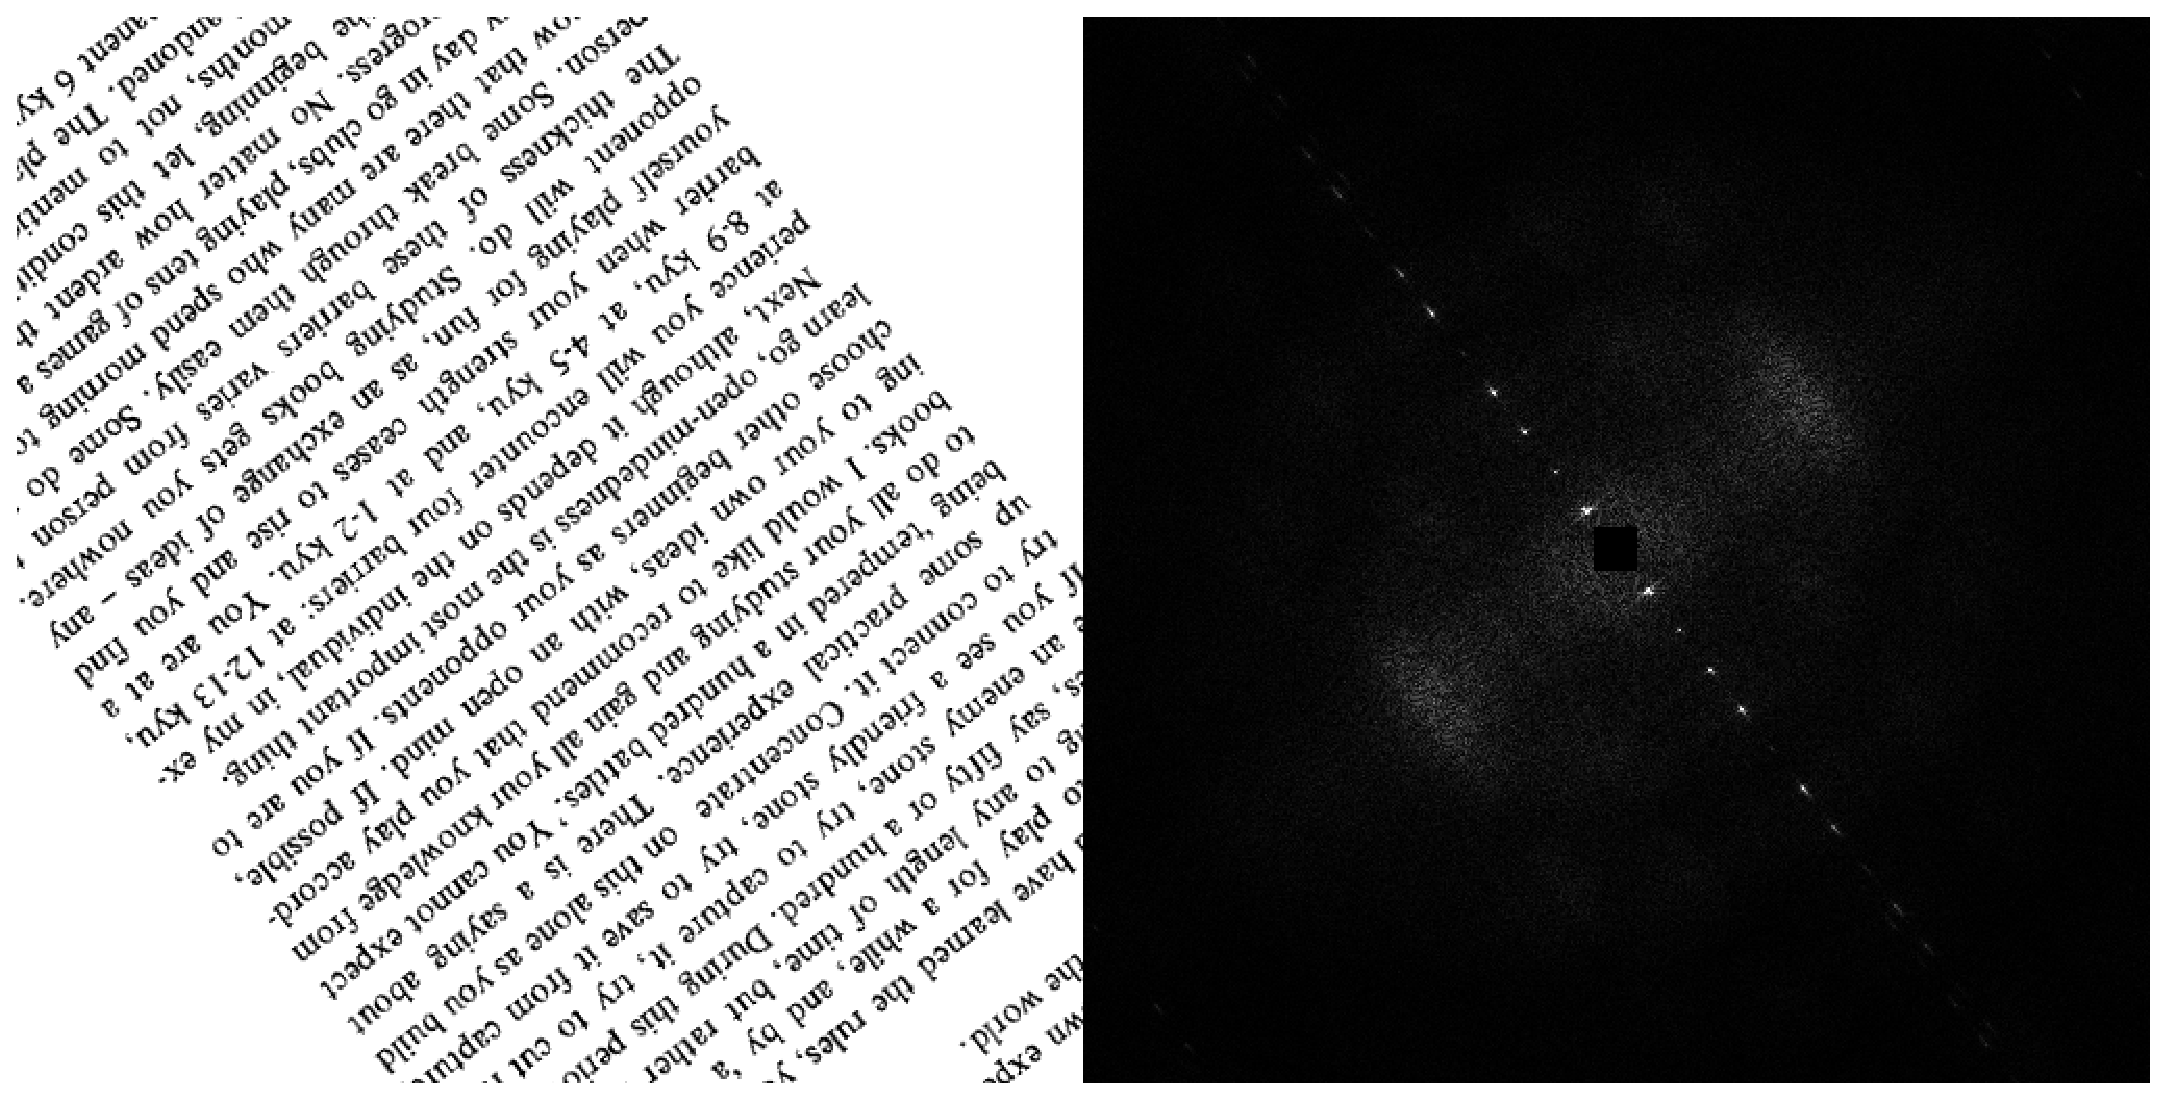
\includegraphics[width=150mm]{u04/task1.eps}
%\end{center}
%\caption{Rotationserkennung}
%\end{figure}

\begin{lstlisting}[caption=Ausgabe]
Paste some output here
\end{lstlisting}


\section*{Aufgabe 2 - Haar Wavelet Transformation}
Da sich bei der (Haar) Wavelet Transformation um eine lineare Transformation handelt, die auch
durch eine Matrix-Operation beschrieben werden kann $I_{trans} = W * (W*I)^{T}$, liegt die
Hauptarbeit in der Generierung der Wavelet-Matrix.
\\
F\"ur die Erstellung der Matrix w\"ahlten wir den ``Inversen Ansatz''. Daf\"ur implmentierten wir
eine rekursive Funktion f\"ur die inverse Wavelet-Transformation. Dieser \"ubergeben wir sequentiell die $N$ Zeilenvektoren der Identit\"atsmatrix $I(N)$ und setzen aus den Ergebnissen die inverse
Wavelet-Matrix zusammen.
\\
Nachfolgende Abbildung zeigt das Ergebnis unserer Durchf\"uhrung, wobei die Werte der Wavelet-
Matrix zur besseren Visualisierung verst\"arkt wurden.

\begin{figure}[H]
\begin{center}
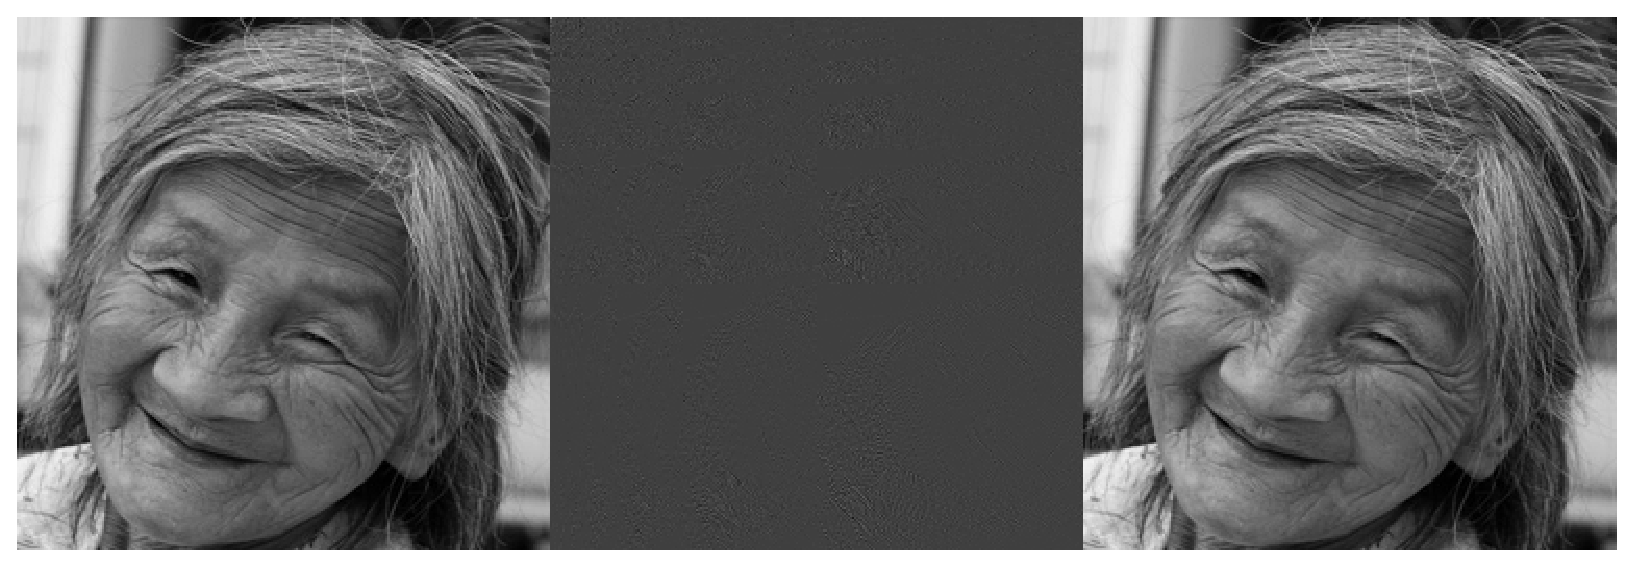
\includegraphics[width=150mm]{u04/task2.eps}
\end{center}
\caption{Verlustfreie Wavelet Transformation}
\end{figure}


\section*{Aufgabe 3 - Wavelet Transformation mit Verlust}
In unserem Beispiel haben wir etwa 40.000 Elemente der Wavelet-Transformation auf Null gesetzt.
Da sich die Differenz-Werte sowieso in sehr kleinen Bereichen bewegen und nur unter Skalierung 
sichtbar werden, ist ein Unterschied zur verlustfreien Transformation mit blossem nicht sichtbar.
\\
Durch den Informationsverslust treten allerdings Bl\"ocke (die auch ineinander geschachtelt sind)
in der r\"ucktransformierten Ausgabe auf. Diese sind auf die Funktionsweise der Transformation
zur\"uck zu f\"uhren: Jedes Pixel in der Transformation hat Einfluss auf nachfolgende kleinere
Frequenzen, wobei die Werte mit steigender Frequenz in der Regel kleiner werden. Mit h\"oherem
Schwellwert w\"urde so also auch die Blockgr\"osse steigen. 

\begin{figure}[H]
\begin{center}
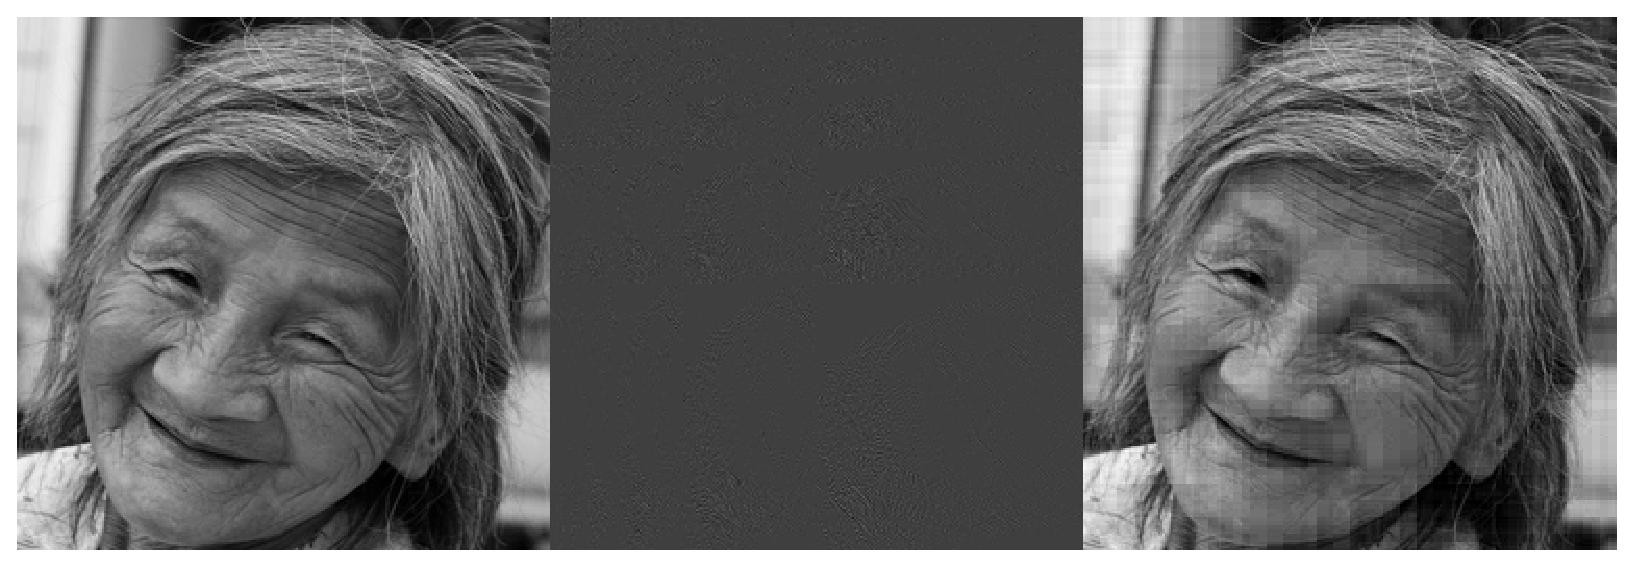
\includegraphics[width=150mm]{u04/task3.eps}
\end{center}
\caption{R\"ucktransformation nach Verlust}
\end{figure}

\end{document}
